\clearpage
\chapter{MÉTHODE ET TECHNIQUES UTILISÉES POUR L'ANALYSE DES SENTIMENTS ET DES ÉMOTIONS}




\textbf{Introduction}\par
Ce chapitre se concentre sur les méthodes et techniques utilisées dans notre projet d'analyse des sentiments. Nous explorerons les approches spécifiques que nous avons adoptées pour extraire des informations significatives à partir de données textuelles, en mettant en lumière les outils et les modèles que nous avons utilisés pour analyser les opinions, les attitudes et les émotions exprimées dans le langage humain. En examinant ces méthodes, nous visons à fournir un aperçu clair et concis de notre approche d'analyse des sentiments, en soulignant les choix et les considérations qui ont guidé notre travail.



%%%%%%%%%%%%%%%%%%%%%%%%% CONTENUE %%%%%%%%%%%%%%%%

%%%%%%%%%%%%%%  COLLECTE DES DONNEES %%%%%%%%%%%%%%%%

\section{La collect des données}
La première étape du processus d'analyse des sentiments consiste à collecter des tweets en spécifiant un mot-clé pour récupérer tous les tweets liés à ce mot-clé. Les tweets peuvent être collectés à partir de différentes sources. L'un des moyens est le robot d'exploration de tweets qui collecte une collection de tweets liés en interrogeant le service Web Twitter ceci se voit nommé \textit{'Web Scraping'}. D’une autre façon en peut utiliser l'interface de programme d'application Twitter (API) \footnote{\href{https://developer.x.com/en/docs/twitter-api/v1/tweets/search/overview} {https://developer.x.com/en/docs/twitter-api/v1/tweets/search/overview}}. Cette API fournie par Twitter et qui donne aux développeurs la possibilité d'utiliser les fonctions de Twitter telles que la récupération de tweets avec le mot-clé et la langue sélectionné. Les tweets collectés seront stockés dans une base de données afin de les classer.

L'objectif le plus important de la collecte de données est de s'assurer que les données recueillies sont fiables et qu'elles regorgent d'informations intéressantes qui peuvent être analysées et transformées en décisions fondées sur des données \cite{questionpro}. 

\section{Exploration des données}
Une bonne connaissance de la santé des données permet d'améliorer la qualité de la fiabilité des informations. C'est à ce moment-là que l'exploration des données entre en jeu.\par
L'exploration des données fournit des informations détaillées sur les caractéristiques des données \cite{astera_blog}. Il s'agit d'identifier les types de données, les valeurs aberrantes, détecter les lignes dupliquées et traiter les données vides. Cet étape aide a comprendre les relations entre les variables et  les distributions des données afin de prendre des décisions éclairées. 

%%%%%%%%%%% PRETRAITEMENT %%%%%%%%%%%%%%%%%%%%%%%
\section{Le prétraitement}
Selon Flo Masdoum \cite{masdoum2023} , " La préparation des données est cruciale ! C'est un peu comme lorsqu'on plante des graines dans un jardin. Avant que les fleurs ne poussent, on prépare le sol et on élimine les mauvaises herbes. Le prétraitement des données dans le NLP, c'est la même idée, mais appliquée aux mots."


%%%%%%%%%%   NETTOYAGE %%%%%%%%%%
\subsection{Le nettoyages des données}
Le potentiel des données propres réside dans l’aisance de leur utilisation. Les données de qualité augmentent l’efficacité, que ce soit dans le cadre du projet pour lequel elles ont été collectées ou bien pour de futurs projets\cite{data_bird_blog}. Le processus de nettoyage des données est similaire pour la plupart des données, parfois il peut varier en fonction de la taille des ensembles de données, leurs nature et l'objectif de l'analyse. 
\subsubsection{Vérification du type des données}
Cet étape permet de vérifier que les ensembles de données ne contient qu’un unique type de données. Il permet d’identifier rapidement les valeurs aberrantes et les sources de problème \cite{data_bird_blog}. 
\subsubsection{ Gestion des valeurs manquantes}
Les valeurs manquantes peuvent entraîner une fausseté dans les résultats de l'analyse. Ils peuvent être traitées de différentes manières, telles que l'imputation par la moyenne, la médiane ou par des algorithmes plus complexes pour prédire les valeurs manquantes.
\subsubsection{Détection et correction des valeurs aberrantes}
Les valeurs aberrantes sont des valeurs extrêmes qui peuvent altérer les résultats de l'analyse. Comment les détecter et les corriger? Il est nécessaire de les repérer et d'évaluer afin de déterminer si elles nécessitent des corrections ou une suppression.
\subsubsection{Gestion des doublons}
Il se peut que lors de la collecte des données, certaines lignes apparaissent deux ou plusieurs fois, surtout lorsque l’on croise différentes sources. Les identifier et les supprimer dès le début permet de réduire le temps d’exécution de toutes les étapes du data cleaning \cite{data_bird_blog}.

%%%%%%%%% La conversion des données %%%%%%%%%
%%%%%%%%%%%% FIGURE %%%%%%%%%%%%%%%%%%%%%ùù
\subsection{Conversion des données}
\begin{figure}[h]
    \centering
    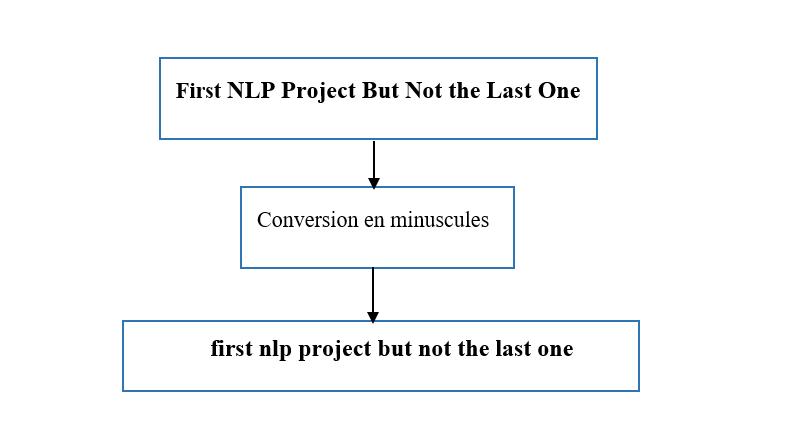
\includegraphics[width=0.7\textwidth]{project_report/figures/Capture d’écran (693).png} 
    \caption{\textit{Conversion des données en minuscules. }} 
    \label{fig:figureConver}
\end{figure}
%%%%%%%%%%%%%%%%%%%%%%%%%%%%%%%%%%%%%%%%%%%%%%%
Cet étape consiste a convertir les tweets en miniscules (Voir l'exemple dans la figure [\ref{fig:figureConver}] pour obtenir une base de données cohérente. Cela évite les problèmes liés à la case car les majuscules et les minuscules peuvent être interprétées différemment par les algorithms. Par exemple, "Hello" et "hello" seraient considérés comme deux mots différents, alors qu'ils devraient être traités comme le même mot. 



%%%%%%%%%%%% Tokenisation %%%%%%%%%%%%%%%%
\subsection{Tokenisation}
La tokenisation permet de décomposer une chaîne de caractères (message ou commentaire) en mots appelés \textit{Tokens }\footnote{un token peut être traduit en tant qu’unité lexicale.}.  Il est encore plus importante dans l’analyse des sentiments que dans d’autres domaines de la NLP, car les informations sur les sentiments sont souvent mal représentée \cite{singh2019nlp}. Cependant de nombreux cas ne sont pas triviaux à traiter \cite{coddity_nlp_blog} :
\begin{itemize}
    \item Les mots avec un trait d’union, exemple : peut être et peut-être qui ont des significations très différentes ;
    \item Les dates et heures qui peuvent être séparées par des points, des slashs, des deux points ;
    \item Les apostrophes ; 
    \item Les caractères spéciaux : émoticônes, formules mathématiques. 
\end{itemize}
La figure [\ref{fig:figureT}] suivante  un exemple de tokenisation, Le passage en minuscule est aussi 
intégré: 


%%%%%%%%%ù FIGURE %%%%%%%%%%%ùùù
\begin{figure}[h]
    \centering
    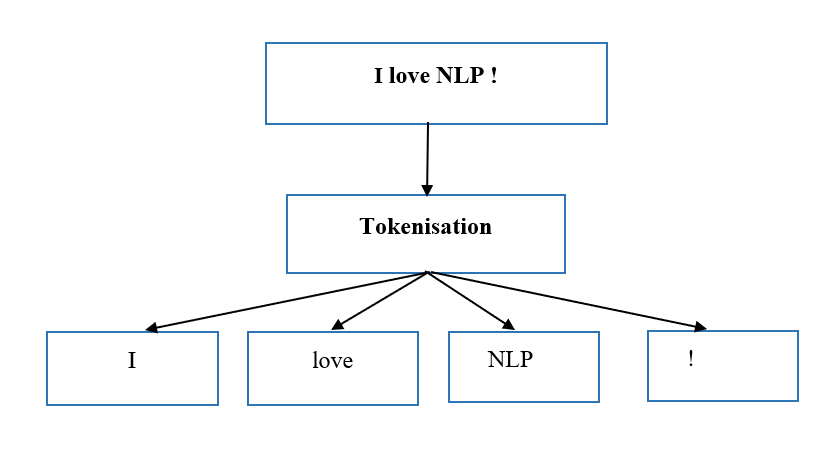
\includegraphics[width=1\textwidth]{project_report/figures/Capture d’écran (692).png} 
    \caption{\textit{Tokenisation}} 
    \label{fig:figureT}
\end{figure}

%%%%%%%%%%% SUPRESSION DES MOTS VIDES %%%%%%%%%%

\subsection{Supressions des mots vides ( StopWords)}
Les mots vides sont les mots qui n'ajoutent pas beaucoup de sens à une phrase. Ils peuvent être ignorés en toute sécurité sans sacrifier le sens de la phrase.  
En NLP, les mots comme "he", "this", "is" .. sont généralement supprimés du texte parce qu’ils peuvent causer du bruit et affecter la précision de l’analyse. Par exemple, Il existe de nombreuses bibliothèques qui fournissent des listes prédéfinies de mots vides dans différentes langues et qui peuvent être utilisées pour les supprimer du texte \cite{5degresNLP}. La figure suivante [\ref{fig:figureVIDE}] présente un exemple avant et après la suppression des mots vides:
%%%%%%%%%%%%%%%%% FIGURE %%%%%%%%%%%%%%%%%%%%
\begin{figure}[h]
    \centering
    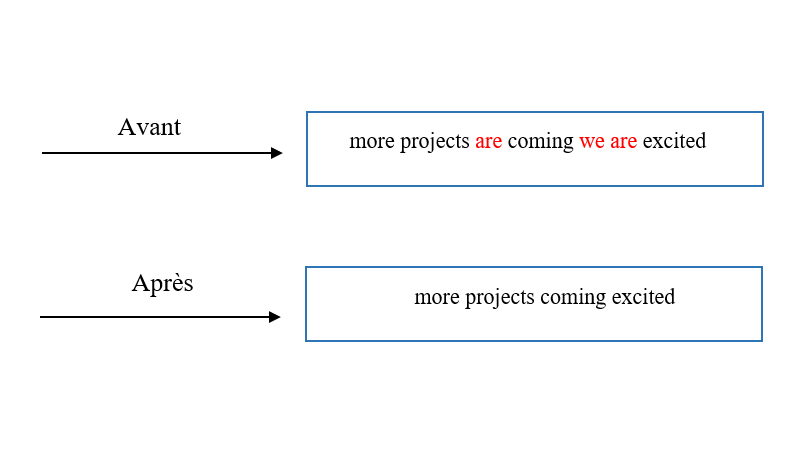
\includegraphics[width=0.7\textwidth]{project_report/figures/Capture d’écran (694).png} 
    \caption{\textit{Avant et après la suppression des mots vides. }} 
    \label{fig:figureVIDE}
\end{figure}

%%%%%%%%%%%%%%%%%%%%%%%%%%%ù


%%%%%%%%%%% GROUPEMENT SEMANTIQUE %%%%%%%%%%%%%
\subsection{Groupement Semantique}
En conséquence, une liste "nettoyée" de mots significatifs, séparés en tokens pour chaque document, est obtenue. Cependant, les mots peuvent être écrits au pluriel, au singulier, ou avec divers accords, tandis que les verbes peuvent être conjugués à différents temps et personnes.
Il est donc nécessaire de réduire les disparités grammaticales en identifiant des formes communes. Pour ce faire, deux approches différentes sont utilisées :
\begin{itemize}
    \item \textbf{La stemmatisation}, qui ignore l'environnement de la phrase. \hfill \\
    \item \textbf{La lemmatisation}, qui tient compte de la situation.
\end{itemize}


%%%%%%%%%%%%%%% Lemmatisation et stemming %%%%%%%%%%%

\subsection{ Stemming et Lemmatisation }
%%%%%%%%%%%%%%%%%%%ù FIGURE LIMMATISATION STEMMATISATION %%%%%

\begin{figure}[h]
    \centering
    \begin{minipage}{0.45\textwidth}
        \centering
        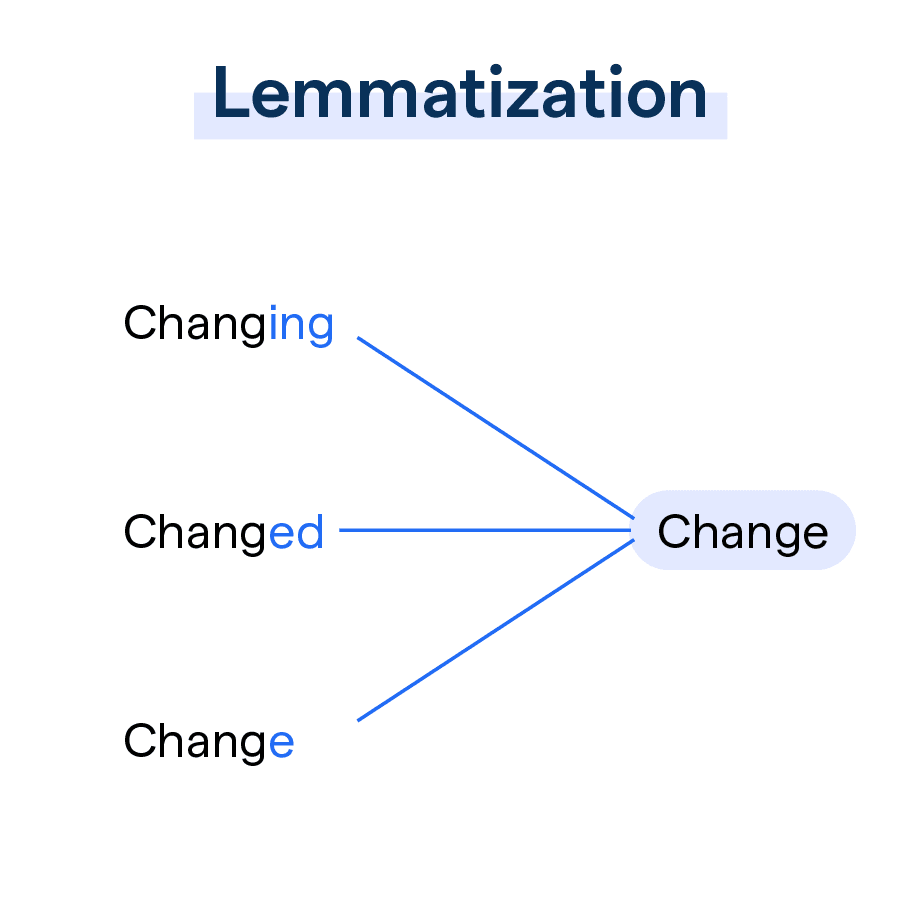
\includegraphics[width=\textwidth]{figures/Lemmatization_5338fc7c3e.png}
        \caption{\textit{Lemmatisation} \cite{botpenguinLemmatization}.}
        \label{fig:figureL}
    \end{minipage}\hfill
    \begin{minipage}{0.45\textwidth}
        \centering
        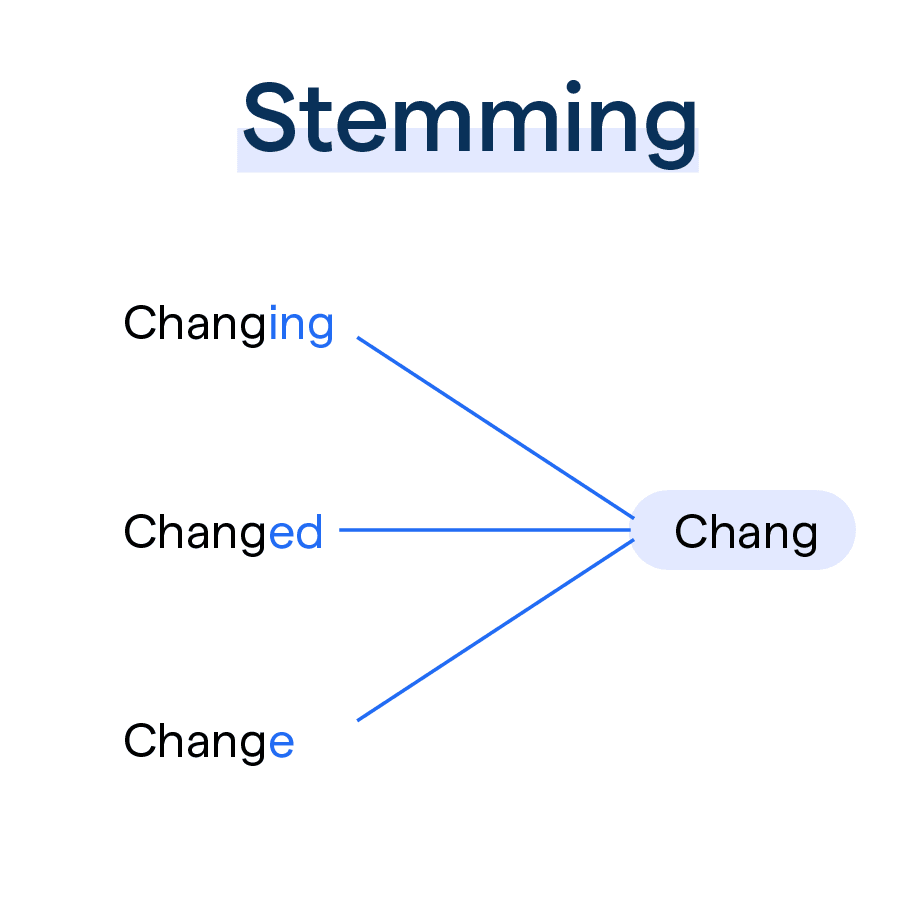
\includegraphics[width=\textwidth]{figures/Stemming_53678d43bc.png}
        \caption{\textit{Stemming }\cite{botpenguinLemmatization}.}
        \label{fig:figureS}
    \end{minipage}
\end{figure}

%%%%%%%%%%%%%%%%%%%%%%%%% TEXTE %%%%%%%%%%%%%%

La lemmatisation \cite{coddity_nlp_blog}, qui prend en considération le contexte dans lequel le mot est écrit, a pour but de trouver la forme canonique du mot, le lemme \footnote{Le lemme correspond à l’infinitif des verbes et à la forme au masculin singulier des noms, adjectifs et articles.}. Par conséquent, elle doit se faire après la transformation des lettres majuscules en minuscules et avant la tokenisation car les mots présents avant et après sont importants pour déterminer la nature du mot.
 Par exemple, cette méthode est capable de faire la différence entre “nous avions” : verbe avoir et “les avions”. \cite{coddity_nlp_blog}.

Le Stemming est  définit comme le processus qui génère des variantes d'un mot racine. En d'autres termes, il réduit un mot à sa forme de base. Cette méthode est utilisée pour simplifier la recherche et normaliser les phrases afin d'améliorer la compréhension (voir l'exemple dans la figure [\ref{fig:figureL}] et [\ref{fig:figureS}])
.
Le stemming et la lemmatisation ne sont pas toujours nécessaires ou bénéfiques pour chaque tâche NLP, et leur utilisation dépend de l’objectif, des données et du langage.




%%%%%%%%%%%%%%%% DIVISION DES DONNEES %%%%%%%%ù
\subsection{La division des données}
Cette étape consiste à séparer l'ensemble de données disponible en plusieurs sous-ensembles pour l'entraînement, la validation et le test des modèles. elle  permet d'évaluer de manière fiable les performances des modèles de machine learning et de deep learning, tout en garantissant qu'ils généralisent bien aux données non vues.

\begin{itemize}
    \item {\textbf{Entraînement :} La majorité des données (par exemple, 70 à 80 \%) est généralement utilisée pour entraîner le modèle. Pendant cette phase, le modèle apprend à partir des données et ajuste ses paramètres pour minimiser l'erreur.
    \item \textbf{Test :} Le reste des données (par exemple, 10 à 20 \%) est utilisé pour tester le modèle final. Ces données sont généralement utilisées une seule fois pour évaluer les performances du modèle après l'entraînement et la validation.}
\end{itemize}


En deep learning, il est généralement préférable de diviser les données en trois ensembles distincts : un ensemble d'entraînement, un ensemble de validation qui sert a évaluer les performances du modèle et un ensemble de test. Cette approche est souvent recommandée pour plusieurs raisons: 

\begin{itemize}
    \item \textbf{Optimisation des hyperparamètres :} En utilisant un ensemble de validation distinct, il est possible d'ajuster les hyperparamètres du modèle de manière plus efficace. Cela permet d'optimiser les performances du modèle sans risque de surajustement aux données d'entraînement.
   
    \item \textbf{Évaluation robuste :} La séparation des données en un ensemble de test distinct garantit une évaluation indépendante des performances du modèle sur des données réellement non vues. Cela permet d'estimer avec précision les performances du modèle dans des conditions réelles d'utilisation.
    
    \item \textbf{Prévention du surajustement :} En évaluant régulièrement les performances du modèle sur l'ensemble de validation pendant l'entraînement, il est possible de détecter et de prévenir le surajustement. Cela permet de garantir que le modèle généralise bien aux données non vues et qu'il n'apprend pas simplement les spécificités des données d'entraînement.
    
    \item \textbf{Comparaison des modèles : }En utilisant un ensemble de test distinct, il est possible de comparer les performances de plusieurs modèles de manière équitable. Cela permet de choisir le modèle le plus performant pour le déploiement en production.
\end{itemize}





%%%%%%%%%%%%%%%%%%%%% VALIDATION CROISEE %%%%%%%%%%%
\section{La validation coisée}
La validation croisée ( en anglais \textit{Cross validation)} est une technique importante en apprentissage automatique et en statistiques pour évaluer la performance d'un modèle et est particulièrement utile lorsque l'ensemble de données est limité. Au lieu de diviser les données en un ensemble de validation fixe et un ensemble de test, la validation croisée divise les données en plusieurs sous-ensembles (appelés "plis", \textit{en anglais "Folds"}) (voir la figure \ref{fig:figureVC}) et utilise chaque pli à tour de rôle comme ensemble de validation, tandis que les autres plis sont utilisés comme ensemble d'entraînement.\par

%%%%%%%%%%%%%%ùù FIGURE %%%%%%%%%%%%%%%%%ùùùù
\begin{figure}[h]
    \centering
    \includegraphics[width=0.7\textwidth]{project_report/figures/validation croisée.png} 
    \caption{\textit{Validation croisée} \cite{towardsdatascience_cross_validation}.}
        \label{fig:figureVC}
 
\end{figure}
%%%%%%%%%%%%%%%%%%% TEXTE %%%%%%%%%%%%%%%%%%ùùù
la validation croisée fonctionne comme la suite :

\begin{itemize}
    \item Division des données en k plis de taille égale (ou approximativement égale).
    \item Entraînement du modèle k fois, en utilisant chaque fois un pli différent comme ensemble de validation et les autres plis comme ensemble d'entraînement.
    \item Calcul de la performance du modèle sur chaque pli de validation et moyenne des performances pour obtenir une estimation globale de la performance du modèle.
\end{itemize}

%%%%%%%%%%%%%%%%%% FEATURE EXTRACTION %%%%%%%%%%

\section{Feature Extraction}

L'utilisation des données textuelles pour la modélisation prédictive, le texte doit être transformé en être utilisable par les algorithmes qui sont conçus pour travailler soit avec des entiers ou numéros réels. La transformation se compose de deux étapes: la tokenisation et la vectorisation.
La tokenisation se réfère à la division du texte en mots, ou tokens, qui représente l'unité atomique d'information. Le texte est donc vu comme une séquence de les jetons et l'étape suivante, la vectorisation, cartographie des jetons à une représentation numérique. Donc, avant d'utiliser les données, elles doivent être codées de manière appropriée. Chaque encodage
technique représente les données d'une manière différente et donc il peut influencer les performances des modèles. Le vecteur de comptage et le vecteur tf-idf ont été identifiés pour satisfaire ce besoin lorsqu'il s'agit de modèles traditionnels. De même, pour les modèles neuronaux, les données ont été encodées avec le vecteur TensorFlow.



%%%%%%%%%%%% BAG OF WORDS %%%%%%%%%%


\subsection{La méthode sac des mots (BagOfWords)}
Le "sac de mots" (ou "\textit{bag of words}" en anglais) est une représentation simplifiée d'un document en traitement automatique du langage naturel (NLP). Dans cette représentation, le texte est considéré comme un "sac" où l'ordre des mots est ignoré, seuls les mots et leur fréquence d'apparition sont pris en compte. \par 
Le principe du sac de mots est plutôt simple. Il se résume en 3 phases :
\begin{itemize}
    \item La décomposition des mots. On appelle cela aussi la tokenisation.
    \item La constitution d’un dictionnaire global qui sera en fait le vocabulaire.
    \item L’encodage des chaînes de caractère par rapport au vocabulaire constitué précédemment.
\end{itemize}

%%%%%%%%%%%%%% COUNT VICTORIZER %%%%%%%%%ù
\subsection{Encodage avec un vecteur de comptage (Count Vectorizer)}

%%%%%%%%%%%%%%%%%%%ùùù FIG %%%%%%%%%%%%%%%%%%%%%%%ùù
\begin{figure}[h]
    \centering
    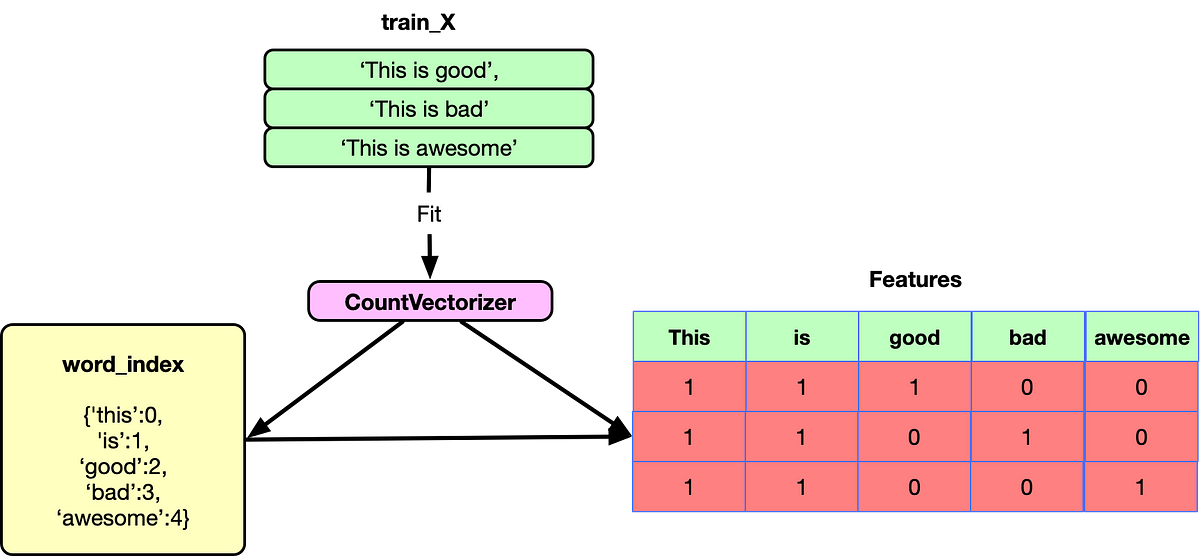
\includegraphics[width=0.7\textwidth]{project_report/figures/count vectorizer.png} 
    \caption{\textit{Vecteur de comptage (CountVectorizer)} \cite{shandeep92}.}
        \label{fig:figureCV}
 
\end{figure}
%%%%%%%%%%%%%%%%%%%%%%%%%%%%%%%%%%%%%%%%%%%%%%%%%

CountVectorizer est inclus dans la bibliothèque Scikit-learn\footnote{\href{https://scikit-learn.org/stable/}{https://scikit-learn.org/stable/}}. Il permet de convertir une série de documents textuels en une matrice de nombres de tokens (Voir l'exemple de la figure [\ref{fig:figureCV}]).  La nouvelle représentation des données présente un nombre de caractéristiques équivalent à la taille du vocabulaire déterminée par l'analyse des données.
En effet, les messages sont constitués de seulement quelques mots par rapport au nombre total de tokens, donc l'utilisation de matrices sparses permet de réduire considérablement la place nécessaire pour les stocker.
Il s'agit d'une méthode simple et basique qui ne prend pas en compte l'ordre des mots dans une phrase et l'importance de chaque mot.
Le CountVectorizer fonctionne comme la suite ( Voir la figure [\ref{fig:figureCV}]): 
\begin{enumerate}
    \item \textbf{Tokenisation :} Le CountVectorizer divise chaque document en mots ou en n-grammes. Un n-gramme est une séquence contiguë de n éléments dans le texte, généralement des mots.
   
    \item \textbf{Construction du vocabulaire :} Le CountVectorizer crée un vocabulaire unique en collectant tous les mots uniques dans l'ensemble des documents. Chaque mot devient une caractéristique dans l'espace vectoriel.
   
    \item \textbf{Création des vecteurs de comptage :} Pour chaque document, le CountVectorizer compte le nombre d'occurrences de chaque mot dans le vocabulaire. Chaque document est ensuite représenté par un vecteur où chaque élément correspond au nombre d'occurrences du mot correspondant dans ce document.
\end{enumerate}



%%%%%%%%%%%%% TF - IDF %%%%%%%%%%%%%%%%%%
\subsection{Encodage avec un vecteur TF-IDF}
Suivant l'idée qu'un mot qui se produit plusieurs fois est moins informatif dans les vecteurs codés que les autres mots qui se produisent moins souvent, une alternative à la vectorisation du nombre est de calculer les fréquences de mots. La méthode la plus populaire qui exploite cette approche est appelée « Fréquence de terme - fréquence inverse de document ». Chaque mot est attribué une valeur destinée à refléter l'importance de ce mot pour un document dans une collection de documents \cite{leskovec2014mining}. Cette valeur, appelée valeur tf-idf, est le produit de la fréquence du terme et de la Fréquence inverse du document.

En définissant $n_t$ comme le nombre de fois où le terme $t$ apparaît dans un document et Nt comme le nombre total de termes dans le document, la fréquence du terme t est définie comme suit :
\begin{equation}
\text{TF}(t) = \frac{n_t}{N_t}
\end{equation}
De la même manière, en définissant $N_d$ comme le nombre total de documents ou de messages dans le cadre de cette thèse, et en définissant $n_{d,t}$ comme le nombre de documents contenant le terme $t$, on peut définir la fréquence inverse des documents comme suit :
\begin{equation}  
\text{IDF}(t) = \log_e\left(\frac{N_d}{n_{d,t}}\right)
\end{equation}
La valeur finale n'est rien d'autre que le résultat de ces deux facteurs :
\begin{equation}
\text{TF-IDF}(t) = \text{TF}(t) \times \text{IDF}(t)
\end{equation}
Il augmente proportionnellement au nombre de fois qu'un mot apparaît dans le document et est contrebalancé par le nombre de documents dans le corpus contenant le mot, ce qui permet de s'adapter au fait que certains mots apparaissent plus fréquemment en général.


%%%%%%%%%%%%%%% N-GRAMMES %%%%%%%%%%%%%%%
\subsection{Encodage avec N-grammes}
L'encodage avec N-grammes dans le cadre du traitement du langage naturel (NLP) consiste à représenter un texte sous forme de séquences de mots contigus de longueur variable, au lieu de simplement considérer des mots individuels. Cette approche permet de capturer les relations entre les mots et le contexte dans lequel ils apparaissent. Il fonctionne comme la suite :

\begin{enumerate}
    \item \textbf{Définition des N-grammes :} Un N-gramme est une séquence de N mots consécutifs dans le texte. Par exemple, un bi-gramme est une paire de mots consécutifs, un tri-gramme est une séquence de trois mots, et ainsi de suite.
    
    \item \textbf{Création des N-grammes :} Pour créer des N-grammes, le texte est divisé en séquences de mots de longueur N. Par exemple, pour un texte "Le chat noir dort", les bi-grammes seraient ("Le", "chat"), ("chat", "noir"), ("noir", "dort"), etc.
    
    \item \textbf{Représentation sous forme de N-grammes :} Chaque N-gramme est ensuite représenté sous forme d'une unité distincte, souvent sous forme de vecteur ou de code numérique, qui capture la fréquence ou la présence de cette séquence dans le texte.
\end{enumerate}

%%%%%%%%%%%%%%%%%%% WORD EMBEDDING %%%%%%%%%%%
\subsection{Incorporation des mots ( Word Embedding)}
Dans son séminaire publié en 2017 pour les cours en ligne de l’université de Stanford, le professeur \textbf{\textit{Christopher Manning}} explique qu’au départ le fait de construire des modèles où les mots sont des éléments atomiques pose rapidement un problème dans le sens où leur représentation se fait via ce que l’on appelle de l’encodage one-hot où le lexique de mots est un long vecteur de 0 et le mot qui nous intéresse est le seul 1 du vecteur. Ceci pose donc un problème, surtout sachant que certains lexiques vocabulaires utilisés en apprentissage profond peuvent compter plusieurs millions de mots (plus de 13 millions de mots pour le Web 1T 5-gram39 corpus de Google par exemple). De plus, la nature atomique de ces représentations fait entièrement abstraction des relations entre les mots (par exemple les synonymes ou les équivalences de genre). Sachant cela, une solution possible consisterait à représenter les mots en tant que vecteurs dont les valeurs représentent d’autres mots qui ont un lien avec ceux-ci et qui sont eux aussi des vecteurs formatés de manière similaire (homme et femme pour reine et roi par exemple). C’est en se basant sur ce principe que l’on peut, via des bibliothèques de word embeddings comme word2vec40 ou GloVe41, construire de phrases composées de vecteurs contextuellement associables et utilisables dans les réseaux de neurones.

La représentation vectorielle est le point de départ de la transformation finale qui permet aux réseaux neuronaux d'apprendre des données d'entrée. On l'appelle l'emballage et il s'agit essentiellement d'une cartographie des données d'entrée sur un vecteur de nombres réels.
Le but des embellissements de mots est de capturer la signification sémantique, en la cartographiant dans un espace géométrique. Ceci est fait en associant un vecteur numérique à chaque mot dans un dictionnaire, de sorte que la distance entre deux vecteurs capturerait une partie de la relation sémantique entre les deux mots associés. L'espace géométrique formé par ces vecteurs est appelé un espace d'incorporation. Idéalement, dans un bon espace d'incorporation, les mots ayant une sémantique similaire sont placés à proximité l'un de l'autre dans l'espace, il est donc possible de classer le sentiment global d'une phrase, en analysant la représentation incrustée des mots qu'elle contient.
Keras offre un moyen simple de générer l'espace d'emballage. Cela se fait par l'intermédiaire de la couche d'intégration. Il prend comme entrée les séquences d'intégrales, qui ont été générées par la vectorisation, et produit la nouvelle représentation exploitée par les couches suivantes.

%%%%%%%%%%%%%%%%%%% MODELS %%%%%%%%%%%%%
\section{Approches basés sur Machine Learning }

%%%%%%%%%%%%%%%%%  REGRESSION %%%%%%%%%%%%%%%%%%%%%%ù
\subsection{Regression logistique}
La régression logistique est un modèle prédictif qui cherche à trouver des associations entre un
vecteur de variables explicatives aléatoires, de nature numérique ou catégorique, \( (x_1, x_2, \ldots, x_k) \),
et une variable dépendante catégorique binaire ou multinomiale \( Y \). Il s’agit tout simplement
d'une transformation non linéaire de la régression linéaire, où on cherche à prédire une classe à
la place d’une valeur numérique continue. Pour ce faire, on utilise une fonction logistique
appelée aussi 'Sigmoïde', pour retourner les probabilités qui sont utilisées pour séparer les
classes à prédire. Exemple : si la probabilité générée par une régression logistique, pour prédire
la tendance d’un titre, est supérieure à 0.5, alors la tendance prédite sera haussière, sinon, elle
est baissière.

Ce modèle produit une courbe logistique, qui est limitée aux valeurs comprises entre 0 et 1.
Soit :
\begin{itemize}
    \item \( Y \) la variable indépendante (à prédire),
    \item \( X = (X_1, X_2, \ldots, X_k) \) les variables dépendantes ou explicatives.
\end{itemize}

Comme le modèle est linéaire, on peut écrire l’équation de régression comme suit :
\[
Y^{(i)} = \beta_0 + \beta_1 x_1 + \beta_2 x_2 + \cdots + \beta_n x_n \quad \text{(3.5)}
\]

Les \( \beta_i \) sont les paramètres du modèle que nous cherchons à estimer pour obtenir notre fonction
de prédiction. On utilise le logarithme naturel des « cotes » de la variable dépendante pour
construire la courbe de la régression logistique, plutôt que la probabilité conditionnelle :
\[
\ln \left( \frac{p(Y = 1 \mid X)}{p(Y = 0 \mid X)} \right) = \beta_0 + \beta_1 x_1 + \beta_2 x_2 + \cdots + \beta_n x_n \quad \text{(3.6)}
\]

\[
p(Y = 1 \mid X) = \frac{e^{\beta_0 + \beta_1 x_1 + \beta_2 x_2 + \cdots + \beta_n x_n}}{1 + e^{\beta_0 + \beta_1 x_1 + \beta_2 x_2 + \cdots + \beta_n x_n}} = \frac{1}{1 + e^{-(\beta_0 + \beta_1 x_1 + \beta_2 x_2 + \cdots + \beta_n x_n)}} \quad \text{(3.7)}
\]


%%%%%%%%%%%% NAIVE BAYES %%%%%%%%%%%
\subsection{Naive Bayes}
Selon \cite{zhang2011novel}, Le classificateur Naive Bayes est l'un des algorithmes les plus puissants pour la classification, et il fonctionne bien même avec des millions d'entrées de données, étant rapide à former.\par
Naive Bayes \cite{konfuzio} est une méthode de classification probabiliste qui utilise le théorème de Bayes pour déterminer l'appartenance la plus probable des objets à une classe connue à l'aide de différentes propriétés. Ce principe peut être utilisé pour les modèles d'IA sous la forme de classificateurs Naive Bayes, qui distinguent par exemple les documents texte de manière algorithmique sur la base des mots qu'ils contiennent. Les propriétés ou caractéristiques qui renseignent l'algorithme sur l'appartenance à une classe sont appelées caractéristiques. Ces variables peuvent être continues, discrètes, catégorielles ou binaires, selon la nature des données d'entrée. \par

"Naïf", \cite{konfuzio} le processus l'est parce qu'il attribue aux caractéristiques une indépendance statistique les unes par rapport aux autres. Elles doivent en outre toutes contribuer dans la même mesure à la classification finale. Le théorème de Bayes, également connu sous le nom de théorème sous-jacent, a été établi par le mathématicien Thomas Bayes au 18e siècle. Il décrit une formule permettant de calculer la probabilité conditionnelle. En d'autres termes, il s'agit de déterminer la probabilité qu'un événement B se produise si l'événement A fait déjà partie de l'histoire. En termes mathématiques, cela se présente comme suit :

%%%%%%%%%%%%%%% THEOREME %%%%%%%%%%%%%%%%%%%%%%%%%%
\begin{theorem} 
Soient \( A \) et \( B \) deux événements, avec \( P(B) > 0 \). La probabilité conditionnelle de \( A \) sachant \( B \) est donnée par :
\[
P(A \mid B) = \frac{P(B \mid A) \, P(A)}{P(B)}
\]
où :
\begin{itemize}
    \item \( P(A \mid B) \) est la probabilité de \( A \) sachant que \( B \) est vrai.
    \item \( P(B \mid A) \) est la probabilité de \( B \) sachant que \( A \) est vrai.
    \item \( P(A) \) est la probabilité a priori de \( A \).
    \item \( P(B) \) est la probabilité a priori de \( B \).
\end{itemize}
\end{theorem}
\par

\subsubsection{Bayésien Naïf Multinomial}
Cette variante est surtout adaptée aux données d'entrée entières et suppose une distribution binomiale pour toutes les variables. Celle-ci décrit le nombre total de résultats positifs d'expériences de Bernoulli répétées. Pour les grands nombres, elle se rapproche de la distribution gaussienne, pour laquelle un type de classificateur spécifique peut être utilisé. L'expression multinomiale est souvent utilisée pour la classification de documents et de textes, où elle compte la fréquence des mots individuels \cite{konfuzio}.
\subsubsection{Bayésien Naïf Complémentaire}
Le modèle de Bayésien Naïf Complémentaire (BNC) est une variation améliorée du modèle de Bayésien Naïf classique, particulièrement adapté aux tâches de classification de texte. Contrairement au Bayésien Naïf traditionnel, qui repose sur une hypothèse d'indépendance forte entre les caractéristiques, le modèle de Bayésien Naïf Complémentaire tente de réduire les biais en tenant compte de l'influence complémentaire des autres classes.

\textbf{Principe et Fonctionnement:} \par
Le Bayésien Naïf Complémentaire se distingue en ajustant les probabilités pour mieux gérer les déséquilibres de classes et les caractéristiques corrélées. Il utilise les informations des autres classes pour améliorer la précision des prédictions, ce qui le rend particulièrement efficace dans des contextes où les classes sont inégales ou où les mots (caractéristiques) ont une forte corrélation.

\textbf{Parmi les avantages de ce modèle: }

\begin{itemize}
    \item \textbf{Meilleure gestion des déséquilibres de classes :} En tenant compte des informations provenant des classes complémentaires, le BNC réduit les biais introduits par les déséquilibres de classes.
    \item \textbf{Amélioration de la précision :} La prise en compte des influences complémentaires permet au modèle de faire des prédictions plus précises, en particulier dans les tâches de classification de texte.
    \item \textbf{Simplicité et efficacité :} Comme le Bayésien Naïf classique, le BNC est relativement simple à implémenter et à exécuter, tout en offrant des améliorations significatives en termes de performance.
    
\end{itemize}


%%%%%%%%%%%%%%  AdaBOOST %%%%%%%%%%%%%%%%%%%%%%
\subsection{AdaBoost}

\begin{figure}[h]
    \centering
    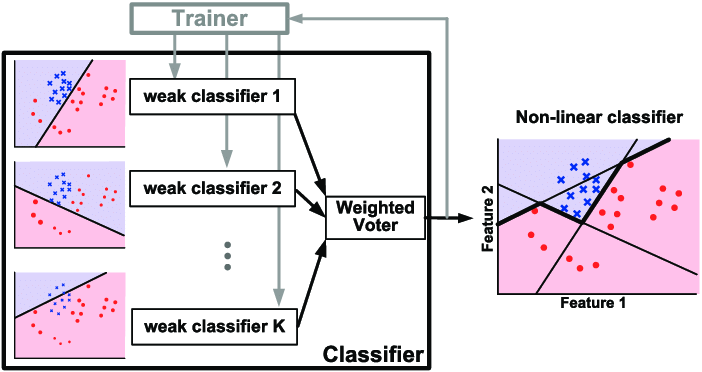
\includegraphics[width=0.7\textwidth]{project_report/figures/Illustration-of-AdaBoost-algorithm-for-creating-a-strong-classifier-based-on-multiple.png} 
    \caption{\textit{AdaBoost} \cite{researchgate2024}.}
        \label{fig:figure3}
 
\end{figure}

Le boosting adaptatif (AdaBoost) est l'un des premiers modèles de boosting\footnote{\href{https://aws.amazon.com/fr/what-is/boosting/}{https://aws.amazon.com/fr/what-is/boosting/}} développés. 
C'est \cite{fineproxy2024} une technique puissante utilisée dans l'apprentissage automatique et la science des données pour créer des algorithmes puissants qui améliorent les capacités prédictives. Il s'agit d'un algorithme de méta-apprentissage d'ensemble de type boosting itératif. L'objectif de l'algorithme AdaBoost est d'améliorer l'exactitude d'un modèle d'apprentissage faible et de créer un modèle amélioré et plus puissant.

AdaBoost fonctionne en combinant un ensemble de modèles faibles \textit{( 'Weak learners' en anglais}, ou "apprenants faibles"), en un seul modèle plus robuste. Chaque apprenant faible est formé sur différents aspects des données, et le modèle final est constitué des contributions de chacun d'entre eux ( Voir la figure \ref{fig:figure3}) . En utilisant plusieurs apprenants faibles, le modèle peut apprendre des modèles plus complexes dans les données qu'un seul apprenant fort ne peut le faire.\par

La clé d'AdaBoost est la sélection des apprenants faibles. Pour sélectionner la meilleure combinaison possible d'apprenants faibles, AdaBoost applique un système de pondération à chaque point de données. Le poids d'un point de données est augmenté s'il a été mal classé par un apprenant faible, et diminué s'il a été correctement classé. Ce système de pondération permet à AdaBoost de se concentrer sur les points de données les plus difficiles à classer et de former un meilleur modèle. \par

AdaBoost est utile pour les problèmes de classification, car il construit un modèle puissant qui peut classer avec précision des points de données, même avec des données bruitées ou incomplètes. AdaBoost est également utile pour les problèmes de régression, car il permet de réduire l'erreur quadratique moyenne en combinant les prédictions individuelles de l'apprenant faible.

\subsubsection{Description de l’algorithme AdaBoost}

Considérons un ensemble d’entraînement \( S = \{(x_1, y_1), \ldots, (x_n, y_n)\} \), où \( x_i \in X \) et \( y_i \in \{-1, 1\} \).

L’algorithme fonctionne comme suit :
\begin{enumerate}
    \item Initialiser les probabilités de chaque donnée \( p_1(i) = \frac{1}{N}, \; \forall \, i = 1, \ldots, N \)
    \item Entrainer le classifieur \( h_j \) avec \( X_j \). (généré à partir de \( X \) selon la probabilité \( p_j(i) \))
    \item Calculer l’erreur de \( h_j \) : \( \epsilon_j = \sum_{i=1}^{N} p_j(i) \delta(y_i \neq h_j(x_i)) \) \\
    (où \( \delta \) est une fonction indicatrice)
    \item Choisir un facteur \( \alpha_t = \frac{1}{2} \ln \left( \frac{1 - \epsilon_t}{\epsilon_t} \right) \)
    \item Mettre à jour la distribution des poids à travers des exemples :
    \[
    D_{t+1}(i) = \frac{D_t(i) \cdot e^{-\alpha_t y_i h_t(x_i)}}{Z_t}, \; \forall \, i \in \{1, 2, \ldots, m\}
    \]
    où \( Z_t \) est un facteur de normalisation.
\end{enumerate}

Résultat : la classe votée \( \forall \, x \), \( C(x) = \text{sign} \left( \sum_{t=1}^{T} \alpha_t \cdot f_t(x) \right) \)





%%%%%%%%%%%%%%%%%%% Nu-SVC %%%%%%%%%%%%%ù
\subsection{Nu-SVC}
Le nu-Support Vector Classification (nu-SVC) est une variante des Support Vector Machines (SVM)\footnote{\href{https://www.ibm.com/topics/support-vector-machine} {https://www.ibm.com/topics/support-vector-machine}}, un algorithme d'apprentissage supervisé largement utilisé pour la classification. Le nu-SVC utilise un paramètre de régularisation appelé "nu" au lieu du paramètre plus courant "C" utilisé dans les SVM traditionnels.

Le paramètre "nu" contrôle à la fois la marge du modèle et le taux d'erreurs tolérées lors de la classification. En d'autres termes, il détermine à la fois la largeur de la marge et le nombre d'erreurs de classification autorisées. Une valeur de "nu" plus basse indique une marge plus large et une tolérance plus élevée aux erreurs, tandis qu'une valeur plus élevée indique une marge plus étroite et une tolérance plus faible aux erreurs.

Le principal avantage du nu-SVC par rapport aux SVM traditionnels réside dans sa capacité à mieux gérer les données déséquilibrées, où les classes à prédire ont des proportions très différentes dans l'ensemble de données. En ajustant le paramètre "nu", le modèle peut être plus flexible dans la manière dont il traite les erreurs de classification, ce qui peut conduire à de meilleures performances dans de telles situations.

Le fonctionnement du nu-Support Vector Classification (nu-SVC) est similaire à celui des Support Vector Machines (SVM) traditionnels, avec une différence principale dans la façon dont il gère la régularisation: 

\begin{enumerate}
    \item \textbf{Séparation des données :} Comme les SVM traditionnels, le nu-SVC vise à trouver un hyperplan dans un espace de dimensions supérieures qui sépare les données en fonction de leurs étiquettes de classe. Cet hyperplan est choisi de manière à maximiser la marge, la distance entre l'hyperplan et les points de données les plus proches de chaque classe, appelés vecteurs de support.
   
    \item \textbf{Optimisation de la marge :} L'objectif est de trouver cet hyperplan de séparation tout en minimisant une fonction de coût. Dans le cas des SVM traditionnels, cette fonction de coût\footnote{La quantification de l'écart entre les prévisions du modèle et les observations réelles du jeu de donnée utilisé pendant l'entraînement} est généralement optimisée en ajustant le paramètre "C". Cependant, dans le nu-SVC, la régularisation est contrôlée par le paramètre "nu". Ce paramètre "nu" contrôle à la fois la largeur de la marge et le nombre d'erreurs de classification autorisées. Une valeur plus faible de "nu" correspond à une marge plus large et à une tolérance plus élevée aux erreurs, tandis qu'une valeur plus élevée de "nu" correspond à une marge plus étroite et à une tolérance plus faible aux erreurs.
   
    \item \textbf{Optimisation et entraînement :} Le modèle nu-SVC est entraîné à l'aide d'un algorithme d'optimisation qui ajuste les paramètres de l'hyperplan pour minimiser la fonction de coût, tout en tenant compte du paramètre "nu" spécifié par l'utilisateur. Cela implique souvent l'utilisation d'algorithmes d'optimisation tels que l'optimisation quadratique ou d'autres méthodes d'optimisation convexe.
   
    \item \textbf{Prédiction :} Une fois entraîné, le modèle nu-SVC peut être utilisé pour prédire les étiquettes de classe des nouveaux exemples en les classant par rapport à l'hyperplan de séparation trouvé pendant l'entraînement.
\end{enumerate}







%%%%%%%%%%%%%%%%% CNN %%%%%%%%%%%%%%%%%%%
\subsection{Les réseaux de neurones convolutif (CNN)}
Les réseaux de neurones convolutifs (également baptisés réseaux de neurones à convolution,\textit{ CNN }ou encore \textit{ConvNets}) sont une forme particulière de réseaux de neurones artificiels multicouches conçus pour traiter des données d’images bidimensionnelles bien qu’ils puissent être utilisés avec des données unidimensionnelles et tridimensionnelles \cite{lopez2020convolutional}. \par
L’architecture des connexions neurales de ces réseaux s’inspire de la structure du cortex visuel des mammifères \cite{lopez2020convolutional}. Ils sont composés de plusieurs couches de neurones combinées avec des fonctions mathématiques à plusieurs paramètres ajustables pouvant prétraiter une quantité d’informations restreinte, comme le montre la figure [\ref{fig:figure14}]:

%%%%%%%%%%%%%%%%%% FIG %%%%%%%%%%%%%%%%%%
\begin{figure}[h]
    \centering
    \includegraphics[width=0.7\textwidth]{project_report/figures/CNN modèle architecture (1).png} 
    \caption{\textit{Réseau de neurones convolutif} \cite{choudhry2024}.}
        \label{fig:figure14}
 
\end{figure}

Un réseau de neurones convolutif est caractérisé par une première couche dite « convolutionnelle » (généralement une à trois premières couches). Cette couche, comme son nom l’indique, est basée sur le principe mathématique de la convolution et tente d’identifier la présence d’un motif ou caractéristiques (par exemple dans une image ou un signal) \cite{lee2018convolutional}.
La convolution est une opération linéaire qui consiste simplement à appliquer un filtre, qui est une matrice bidimensionnelle de poids, à l’entrée du réseau, ce qui entraîne l’activation \cite{lee2018convolutional}. \par
L’application répétée du même filtre à l’entrée produit une carte d’activations appelée cartes des caractéristiques, qui montre la position et l’intensité des caractéristiques détectées dans l’entrées. Le filtre utilisé a une dimension plus petite que celle des données d’entrée. Ce filtre est multiplié via un produit scalaire par un bloc de l’entrée ayant la même tailles que le filtre \cite{lopez2020convolutional}. Le but de l’utilisation d’un filtre plus petit que l’entrée est parce qu’il permet au même filtre (matrice de poids) d’être multiplié par la matrice d’entrée (l’image) plusieurs fois à différents emplacements. Plus précisément, le filtre est systématiquement appliqué à chaque partie ou bloc des données d’entrés de la taille du filtre, de gauche à droite et de haut en bas. Une fois la carte des caractéristiques créée, chacune de ses valeurs peut alors être transférée par non-linéarité, comme la fonction ReLU, dont l’équation est la suivante \cite{lopez2020convolutional}:
\begin{equation}
f(x) = \max(0, x)
\end{equation}
pour tout réel \( x \). \par
L’application systématique d’un même filtre aux données d’entrée s’est avérée efficace : si le filtre est conçu pour détecter un certain type de caractéristiques sur l’entrée, l’application cohérente de ce filtre à l’ensemble de l’image d’entrée permet alors au filtre de détecter cette caractéristique où qu’elle soit sur l’image \cite{lopez2020convolutional}.

%%%%%%%%%%%%%% RNN %%%%%%%%%%%%%%%%
\subsection{Les réseaux de neurones réccurents (RNN)}
Les réseaux de neurones récurrents, également connus sous le nom de RNNs (pour Recurrent Neural Networks en anglais), sont un type de réseaux de neurones permettant aux prédictions antérieures d’être utilisées comme entrées via des états cachés (en anglais hidden states) \cite{wikiRNN}. Ceci est réalisé en propageant l’information dans les deux sens, y compris de couches cachées à la couche d’entrée. C’est ce mécanisme qui les rapproche du vrai fonctionnement du système nerveux, qui n’est pas à sens unique et qui les distingue des autres types de réseaux de neurones grâce à l’utilisation de boucles de rétraction pour traiter une séquence de données qui forme le résultat final, qui lui-même peut être une séquence de données \cite{wikiRNN}. Ces boucles de rétroaction rendent l’information durable, effet généralement équivalent à la mémoire. La figure [\ref{fig:figure1}] ci-dessous illustre une représentation d’un RNN :
%%%%%%%%%%%%%%%%%% FIG %%%%%%%%%%%%%%%%%%
\begin{figure}[h]
    \centering
    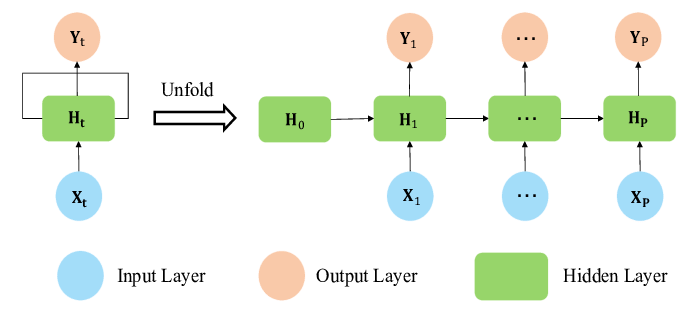
\includegraphics[width=0.7\textwidth]{project_report/figures/1_hpuxp7JFtcqysvkF_oJdRA.png} 
    \caption{\textit{Réseaux de neurones réccurents } \cite{choudhry2024}.}
        \label{fig:figure1}
 
\end{figure}

Le bloc étiqueté $A$ est un simple réseau de neurones à propagation directe déjà familier. Le côté droit de la figure montre le réseau $A$ à chaque pas de temps $t$, c’est-à-dire à $t = 0$, l’entrée $x_0$ est assimilée par le réseau pour générer la sortie $h_0$, l’entrée du pas de temps suivant est donc $x_1$. Seulement, il y a une entrée additionnelle du pas de temps précédent à partir du bloc $A$. Ainsi, le réseau neural prend en compte non seulement l’entrée actuelle, mais dispose aussi du contexte des entrées précédentes \cite{wikiRNN}. La figure suivante représente un échantillon du réseau neuronal récurrent, c’est-à-dire une unité unique du RNN :


Les formules régissant le calcul de la sortie d’une unité du RNN à l’instant \( t \) sont les suivantes \cite{wikiRNN}:
\begin{align}
A_t &= g(W_{ax} x_t + W_{aa} A_{t-1} + b_a) \\
h_t &= g(W_{ya} A_t + b_y)
\end{align}

Où :
\begin{itemize}
  \item \( A \) est la sortie de la couche cachée.
  \item \( g\)est la fonction d’activation.
  \item \( W \) est la matrice de poids.
  \item \( x \) est l’entrée.
  \item \( h \) est la sortie à un pas de temps \( t \).
  \item \( b \) est le biais.
\end{itemize}

Pour le RNN, la disparition du gradient est un problème majeur, puisque les réseaux de neurones qui ne peuvent plus être entrainés convenablement perdront inévitablement leurs performances. Cette disparition se produit dans les réseaux de neurones multicouches utilisés pour traiter des données complexes \cite{salehinejad2018recent}. Ajouter efficacement ces paramètres dès les premières couches nécessite beaucoup de temps et de ressources. Une façon de résoudre ce problème consiste en l’utilisations d’unités \textit{LSTM} \textit{(Long Short-Term Memory)} à mémoire court terme étendue. Les réseaux de neurones récurrents dotés d’unités LSTM sont capables de classer les données dans des cellules de mémoire à long terme ou à court terme. De cette manière, ils peuvent faire la distinction entre les données importantes devant être mémorisées et réinjectées dans le réseau et les données devant être « oubliées » \cite{salehinejad2018recent}.


%%%%%%%%%%%%%%% LSTM %%%%%%%%%

\section{Réseaux de neurones récurrents modernes(LSTM)}
Bien que les réseaux de neurones récurrents soient largement utilisés, ils ne sont pas suffisamment efficaces pour résoudre les problèmes actuels d'apprentissage de séquences. Par exemple, compte tenu de l'instabilité numérique lors du calcul du gradient, les réseaux de neurones modernes sont utilisés beaucoup plus souvent dans la pratique \cite{salehinejad2018recent}. \par
\subsection{Long Short-Term Memory (LSTM) }
%%%%%%%%%%%%%%%%%%%%ù FIG 

%%%%%%%%%%%%%%%%%%%%%%%%%%%%
Les cellules \textit{Long Short-Term Memory} sont conçues pour surmonter le problème de la disparition du gradient (en anglais,\textit{ Vanishing Gradient}) dans les réseaux de neurones récurrents et leur permettre de conserver les informations plus longtemps par rapport aux RNNs traditionnels \cite{hochreiter1997}. \par
Les LSTM ont la capacité de maintenir une erreur constante qui leur permet de continuer l’apprentissage sur de nombreux pas de temps et se propager à travers les couches \cite{hochreiter1997}.\par


Les LSTM disposent d’une structure en chaine qui contient quatre réseaux de neurones et différents blocs de mémoires appelés \textit{cellules}. Les informations sont sauvegardées par les cellules et les manipulations de la mémoire sont effectuées par ce qu’on appelle des « portes », qui sont des mécanismes internes permettant de réguler le flux d’information \cite{graves2012}, comme nous pouvons le constater dans l’architecture de la cellule LSTM représentée dans la figure ci-dessous :

%%%%%%%%%ù FIGURE %%%%%%%%%%%ùùù
\begin{figure}[h]
    \centering
    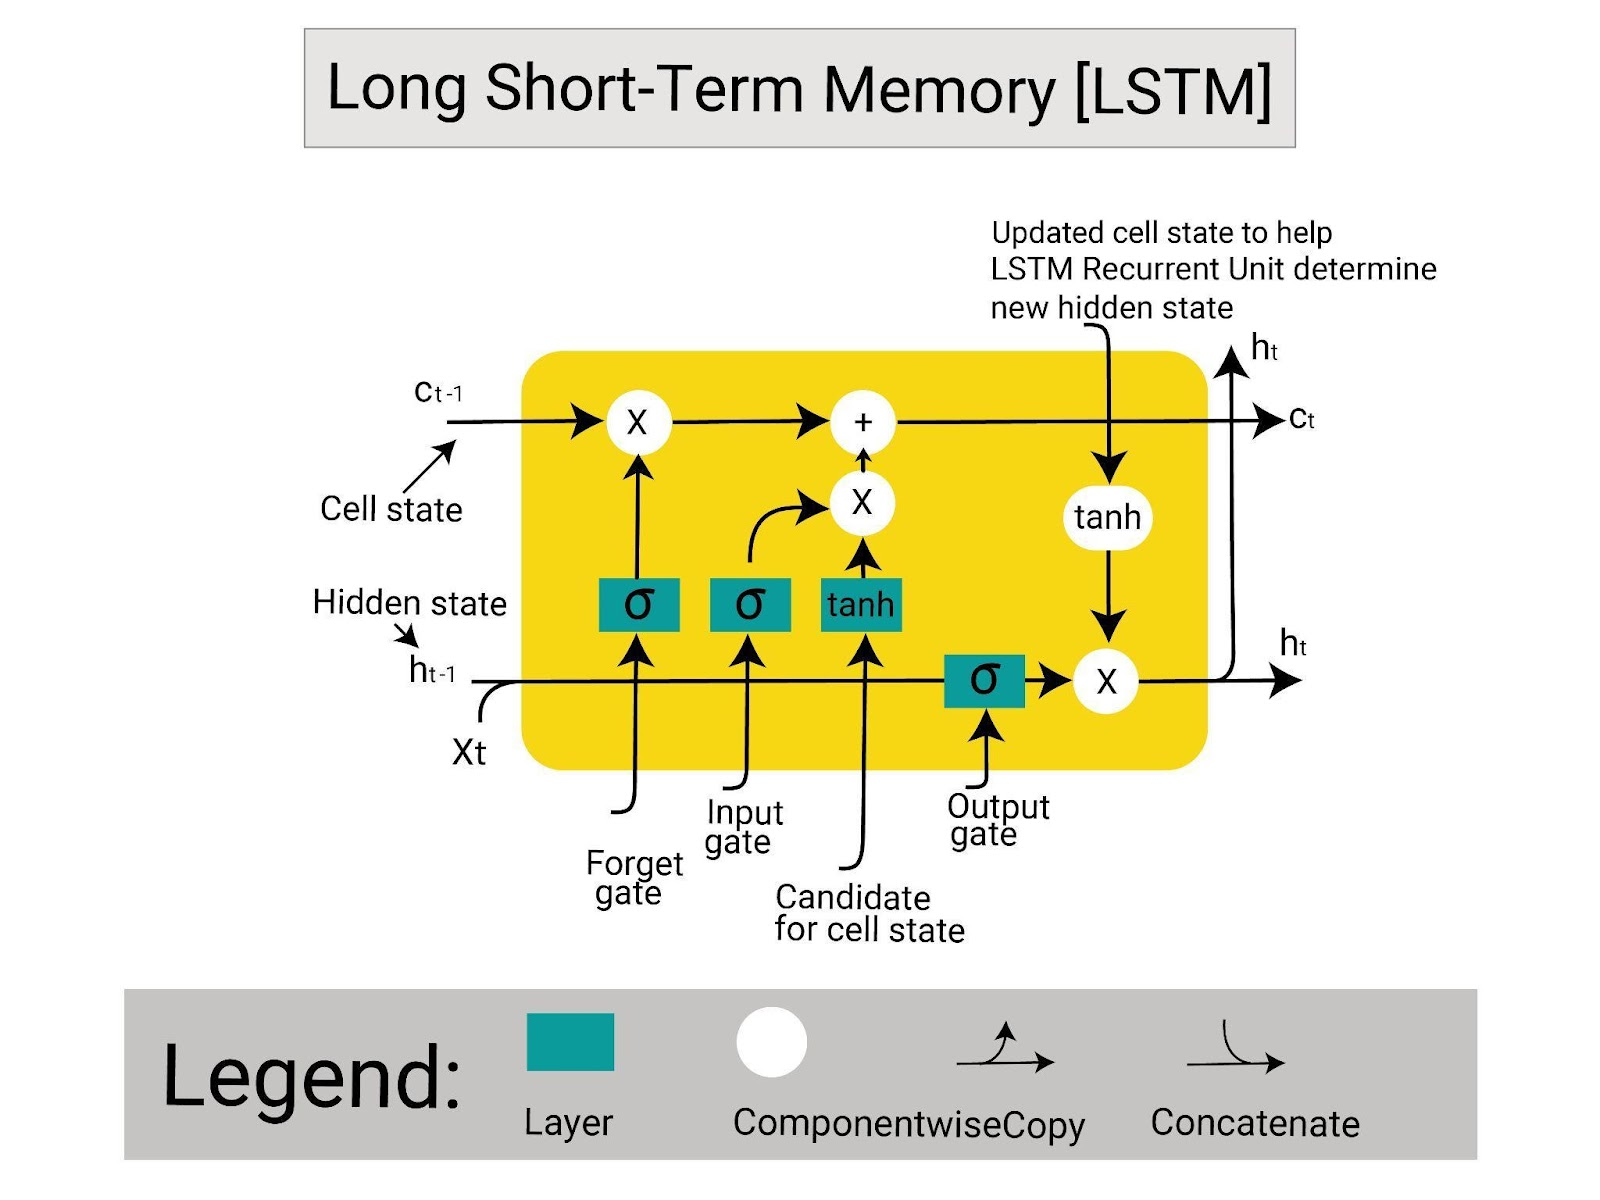
\includegraphics[width=0.7\textwidth]{project_report/figures/image-6.jpeg} 
    \caption{\textit{Long Short-Term Memory}  \cite{liberiangeek2024}.}
        \label{fig:figureLSTM}
 
\end{figure}



%%%%%%%%%%%%%%%%%% EVALUATION %%%%%%%%%%%%%%%
\section{Evaluation}
L'exactitude, la précision, le score F1 et le rappel sont des mesures communes pour mesurer les performances des modèles de classification.
Pour rappeler leur définition, il est utile d'introduire la matrice de confusion. C'est une matrice qui résume combien d'éléments d'entrée ont été correctement classés et combien n'en ont pas. Chaque ligne de la matrice représente les instances d'une classe prédite tandis que chaque colonne représente des instances dans une classe réelle. Les éléments classifiés relèvent des catégories suivantes :

\begin{itemize}
    \item Vrai Positive \textbf{(TP)} : nombre de tweets positifs classés correctement. \par
    \item Faux positive \textbf{(FP) }: nombre de tweets négatifs classés à tort comme positifs.\par
    \item Vrai Négative \textbf{(TN) }: nombre de tweets négatifs classés correctement.\par
    \item Faux Négative \textbf{(FN)} : nombre de tweets positifs classés à tort comme négatifs.\par
\end{itemize}


%% Table 



\begin{table}[h!]
    \centering
    \begin{tabular}{|c|c|c|}
        \hline
        & \multicolumn{2}{c|}{Classe Prédite} \\ \hline
        & Positif Prédit & Négatif Prédit \\ \hline
        Positif Réel & Vrai Positive (TP) & Faux Négative (FN) \\ \hline
        Négatif Réel & Faux Positif (FP) & Vrai Négatif (TN) \\ \hline
    \end{tabular}
    \caption{Matrice de confusion}
    \label{tab:confusion_matrix}
\end{table}
%%%%%%%  






%%%%%%%%%%%%%% PRECISION %%%%%%%%%%%%%%%%%%
\subsection{Précision}
La précision (\textit{Precision}) \cite{vilares2015lexicon} est également appelée valeur prédite positive, mesure la justesse
du modèle. Une précision plus élevée indique moins de FP. Mathématiquement, il est
défini comme : 
\begin{equation}
\text{Précision} = \frac{TP}{TP + FP}
\end{equation}
où :
\begin{itemize}
  \item $TP$ est le nombre de vrais positifs,
  \item $FP$ est le nombre de faux positifs.
\end{itemize}

%%%%%%%%%%%%%%% RAPPEL %%%%%%%%%%%%%
\subsection{Rappel}
Le rappel (\textit{Recall}) \cite{vilares2015lexicon}  est également connu sous le nom de sensibilité, mesure les cas positifs correctement classés par le modèle.  une valeur de rappel élevée signifie que peu de cas positifs sont mal classés comme négatifs. Le rappel peut être calculé à l'aide de la formule suivante: 

\begin{equation}
\text{Rappel} = \frac{TP}{TP + FN}
\end{equation}
où :
\begin{itemize}
  \item $TP$ est le nombre de vrais positifs,
  \item $FN$ est le nombre de faux négatifs.
\end{itemize}

%%%%%%%%%%%%%%%% EXACTITUDES %%%%%%%%%%%%%%%%%%%%
\subsection{Exactitudes}
L’exactitudes (\textit{Accuracy})  \cite{sebastiani2002text} utilisée comme mesure pour les techniques de catégorisation. Les valeurs de exactitudes, cependant, sont beaucoup moins réticentes aux variations du nombre de décisions correctes que la précision et le rappel. Cette technique est
représentée sous la forme suivante :
\begin{equation}
\text{Exactitude} = \frac{TP + TN}{TP + FP + TN + FN}
\end{equation}
où :
\begin{itemize}
  \item $TP$ est le nombre de vrais positifs,
  \item $TN$ est le nombre de vrais négatifs,
  \item $FP$ est le nombre de faux positifs,
  \item $FN$ est le nombre de faux négatifs.
\end{itemize}


%%%%%%%%%%%%%%%%%%%% F1 SCORE %%%%%%%%%%%ù
\subsection{Le score F1}
Le score F1 (\textit{F1-Score}) ou la mesure F1 \cite{vilares2015lexicon} est la moyenne harmonique de la précision et du rappel. Le score F peut être calculé comme suit :
\begin{equation}
\text{Score F1} = 2 \times \frac{\text{Précision} \times \text{Rappel}}{\text{Précision} + \text{Rappel}}
\end{equation}
où :
\begin{itemize}
  \item $\text{Précision}$ est la précision,
  \item $\text{Rappel}$ est le rappel.
\end{itemize}
\vspace{0.5cm}
\textbf{Conclusion}\\
En conclusion, ce chapitre a mis en lumière les méthodes et techniques clés utilisées dans notre projet. Des modèles d'apprentissage automatique avancés aux méthodes de prétraitement textuel, nous avons exploré une gamme diversifiée d'approches visant à capturer la richesse et la complexité des données textuelles. Ces méthodes et techniques, combinées à une compréhension approfondie du domaine et des besoins spécifiques de notre projet, ont permis d'obtenir des résultats prometteurs dans l'analyse des sentiments.






